\documentclass{article}

\usepackage{amsmath,amsfonts}
\usepackage[margin=3cm]{geometry}

\usepackage{multirow}

\usepackage{hyperref}
\hypersetup{
    colorlinks = true,
    linkcolor  = blue,
    urlcolor   = blue,
    citecolor  = blue
}

\usepackage{longtable}

\usepackage[numbers]{natbib}
\defcitealias{Cormen}{Cormen}
\defcitealias{Goodrich}{Goodrich}

\usepackage[usenames, dvipsnames]{xcolor}

\usepackage{tikz}
\usetikzlibrary{shapes}
\tikzstyle{bplus}=[rectangle split, rectangle split horizontal,rectangle split ignore empty parts,draw,scale=0.75]
\tikzstyle{every node}=[bplus]

\usepackage{listings}
\lstdefinestyle{pseudo}
{
    keywordstyle = [1]{\normalfont\bfseries},
    keywordstyle = [2]{\normalfont\it},
    keywordstyle = [3]{\normalfont},
    morekeywords = [1]{repeat, for, to, return, if},
    morekeywords = [2]{H, max, childInd, i, j, k, d, e, pos},
    morekeywords = [3]{let},
    morecomment = [l][\color{BrickRed}\it]{//}
}

\title{Solutions for Data Structures and Algorithms Spring 2023 — Problem Sets}
\author{By Dmitriy Okoneshnikov, B22-DSAI-04}

\begin{document}

\maketitle

\section*{Week 9. Homework 2}

\setcounter{section}{3}
\subsection{Dynamic Programming (20 points)}

Two cities A and B are connected by a highway. Your task is to place shopping centers along the highway in an efficient way, maximizing estimated revenue. Possible locations of shopping centers along the highway are given by $N$ numbers $x_1, x_2, ..., x_N$. Each number specifies the number of kilometers from city A to that location on a highway. For each position $x_i$ we also know in advance the estimated revenue $r_i$ that we get if we place a shopping center there. There is a restriction that no two shopping centers can be placed within $d$ kilometers of each other. The highway length is $H$ kilometers and we have $0 < x_1 < x_2 < ... < x_n < H$.

For example, if we have 4 locations $x_1 = 5, x_2 = 10, x_3 = 14, x_4 = 15$ with estimated revenue $r_1 = 80, r_2 = 150, r_3 = 60, r_4 = 75$ and $d = 6$ then the maximum revenue is 155 when we place two shopping center at locations $x_1 = 80, x_4 = 15$.

Describe a general algorithm for any number $N$ of available locations, any length of the highway $H$:
\begin{enumerate}
    \item Write down pseudocode for a recursive algorithm that solves the problem.
   
    \textbf{Answer.}

    
    
    \item Provide asymptotic worst-case time complexity of the recursive algorithm

    \textbf{Answer.} $O(2^n)$
    
    \item Identify overlapping subproblems.

    \textbf{Answer.}
    
    \item Write down pseudocode for the optimized algorithm that solves the problem using dynamic programming (top-down or bottom-up). The algorithm should compute both the maximum estimated revenue \textbf{and} the specific locations where shopping centers should be placed.

    \textbf{Answer.}
    
    \item Provide asymptotic worst-case time complexity of the dynamic programming algorithm.

    \textbf{Answer.} $O(H)$
    
\end{enumerate}

\subsection{B-Trees (15 points)}

Insert the following $\langle key, value \rangle$ items into an initially empty B-tree [\citetalias{Cormen}, Chapter 18] with minimum degree $t = 2$. Show the state of the tree after every 5 insertions (your answer must contain exactly 4 trees):
\begin{enumerate}
    \item $\langle 17, R \rangle, \langle 6, T \rangle, \langle 9, I \rangle, \langle 7, S \rangle, \langle 12, U \rangle$

    \textbf{Answer.}
    
    \begin{center}
        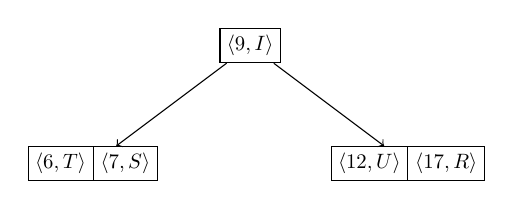
\begin{tikzpicture}
        \tikzstyle{level 1}=[sibling distance=40mm]
        \node {$\langle 9, I \rangle$} [->]
        child { node {$\langle 6, T \rangle$ \nodepart{two} $\langle 7, S \rangle$} }
        child { node {$\langle 12, U \rangle$ \nodepart{two} $\langle 17, R \rangle$} }
        ;\end{tikzpicture}
    \end{center}
    
    \item $\langle 1, D \rangle, \langle 15, D \rangle, \langle 19, E \rangle, \langle 2, A \rangle, \langle 3, S \rangle$

    \textbf{Answer.}
    
    \begin{center}
        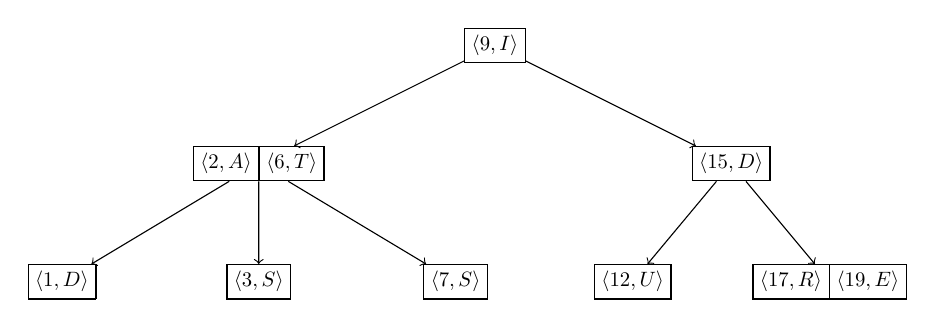
\begin{tikzpicture}
        \tikzstyle{level 1}=[sibling distance=60mm]
        \tikzstyle{level 2}=[sibling distance=25mm]
        \node {$\langle 9, I \rangle$} [->]
        child { node { $\langle 2, A \rangle$ \nodepart{two} $\langle 6, T \rangle$ } 
            child { node { $\langle 1, D \rangle$ } }
            child { node { $\langle 3, S \rangle$ } }
            child { node { $\langle 7, S \rangle$ } }
        }
        child { node {$\langle 15, D \rangle$} 
            child { node { $\langle 12, U \rangle$ } }
            child { node { $\langle 17, R \rangle$ \nodepart{two} $\langle 19, E \rangle$ } }
        }
        ;\end{tikzpicture}
    \end{center}
    
    \item $\langle 10, R \rangle, \langle 8, T \rangle, \langle 4, T \rangle, \langle 5, A \rangle, \langle 20, S \rangle$

    \textbf{Answer.}

    \begin{center}
        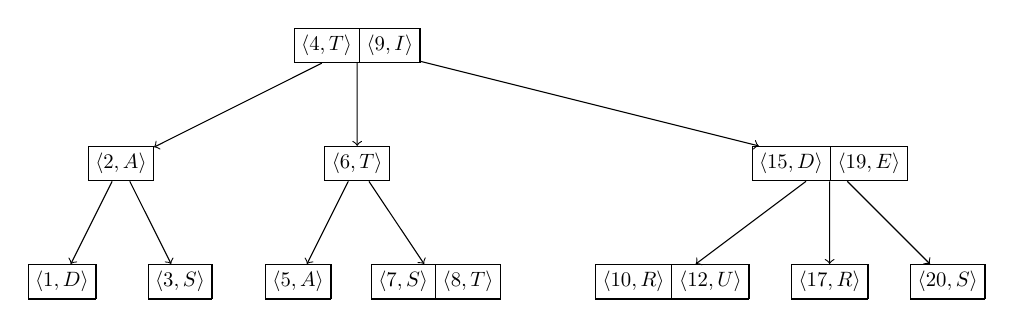
\begin{tikzpicture}
        \tikzstyle{level 1}=[sibling distance=40mm]
        \tikzstyle{level 2}=[sibling distance=25mm]
        \node {$\langle 4, T \rangle$ \nodepart{two} $\langle 9, I \rangle$} [->]
        child[sibling distance=30mm] { node { $\langle 2, A \rangle$ } 
            child[sibling distance=15mm] { node { $\langle 1, D \rangle$ } }
            child[sibling distance=15mm] { node { $\langle 3, S \rangle$ } }
        }
        child[sibling distance=40mm] { node { $\langle 6, T \rangle$ }
            child[sibling distance=15mm] { node { $\langle 5, A \rangle$ } }
            child[sibling distance=20mm] { node { $\langle 7, S \rangle$ \nodepart{two} $\langle 8, T \rangle$ } }
        }
        child[sibling distance=60mm] { node { $\langle 15, D \rangle$ \nodepart{two} $\langle 19, E \rangle$ } 
            child[sibling distance=20mm] { node { $\langle 10, R \rangle$ \nodepart{two} $\langle 12, U \rangle$ } }
            child[sibling distance=15mm] { node { $\langle 17, R \rangle$ } }
            child[sibling distance=15mm] { node { $\langle 20, S \rangle$ } }
        }
        ;\end{tikzpicture}
    \end{center}
    
    \item $\langle 14, T \rangle, \langle 18, Y \rangle, \langle 11, U \rangle, \langle 13, C \rangle, \langle 16, U \rangle$

    \textbf{Answer.}

    \begin{center}
        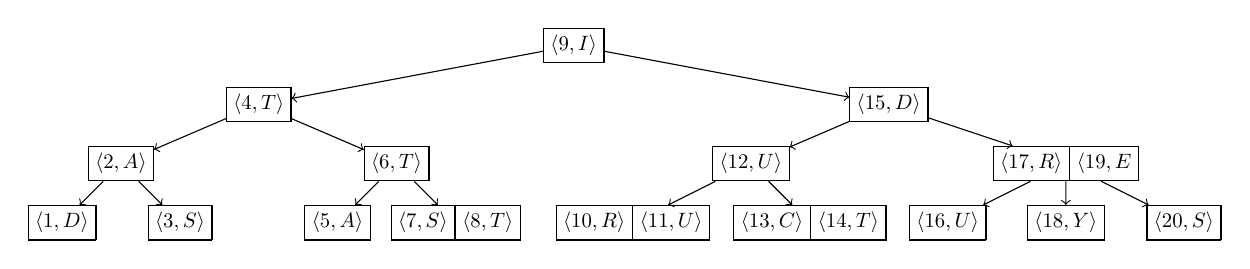
\begin{tikzpicture}[scale=0.5]
        \tikzstyle{level 1}=[sibling distance=160mm]
        \tikzstyle{level 2}=[sibling distance=70mm]
        \tikzstyle{level 3}=[sibling distance=30mm]
        \node {$\langle 9, I \rangle$} [->]
        child { node { $\langle 4, T \rangle$ } 
            child { node { $\langle 2, A \rangle$ } 
                child { node { $\langle 1, D \rangle$ } }
                child { node { $\langle 3, S \rangle$ } }   
            }
            child { node { $\langle 6, T \rangle$ } 
                child { node { $\langle 5, A \rangle$ } }
                child { node { $\langle 7, S \rangle$ \nodepart{two} $\langle 8, T \rangle$ } }
            }
        }
        child { node { $\langle 15, D \rangle$ }
            child { node { $\langle 12, U \rangle$ } 
                child[sibling distance=60mm] { node { $\langle 10, R \rangle$ \nodepart{two} $\langle 11, U \rangle$ } }
                child { node { $\langle 13, C \rangle$ \nodepart{two} $\langle 14, T \rangle$ } }
            }
            child[sibling distance=90mm] { node { $\langle 17, R \rangle$ \nodepart{two} $\langle 19, E$ } 
                child { node { $\langle 16, U \rangle$ } }
                child { node { $\langle 18, Y \rangle$ } }
                child { node { $\langle 20, S \rangle$ } }
            }
        }
        ;\end{tikzpicture}
    \end{center}
    
\end{enumerate}

\subsection{Binary Search Trees with Equal Keys (15 points)}

Equal keys pose a problem for the implementation of Binary Search Trees. We propose to improve insertion into a Binary Search Tree by testing for each node whether inserted key is equal to the key stored in the inspected nodes. If equality holds, then we employ one of the following strategies.

For each strategy, find the asymptotic time complexity of inserting $n$ items with identical keys into an initially empty binary search tree. Justify your answer for each strategy.
\begin{enumerate}
    \item No special strategy, use regular insertion algorithm.
    
    \textbf{Solution.}

    With no specials strategies it would be just an ordinary insertion. Every time when a new element gets inserted we would always go to one side of a tree. At the end we would have a singly linked list, so insertion of $n$ elements would have time complexity of $O(n \cdot n) = O(n^2)$.
    
    \textbf{Answer.} $O(n^2)$
    
    \item Keep a boolean flag at every node. This flag determines whether to go left or right when inserting an item with the key equal to the one in the node. Every time we visit the node with the key equal to node’s key, we switch the flag.

    \textbf{Solution.}

    This strategy allows our tree to balance itself, therefore, the height of this tree is $O(\log{n})$. The time complexity is $O(n\log{n})$.

    \textbf{Answer.} $O(n\log{n})$
    
    \item Keep a list of values with equal keys in each node. Insert the item into that list.

    \textbf{Solution.}
    
    This will result our tree to have only one node with a list that will have $n$ elements in the end. Insertion into a list can be done in $O(1)$, therefore, the time complexity would be $O(n \cdot 1) = O(n)$

    \textbf{Answer.} $O(n)$
    
    \item Randomly choose either left of right. For this strategy, show both the worst-case time complexity, and informally derive the expected time complexity.

    \textbf{Solution.}

    In the worst case every element will be inserted into one of the side of the tree, so it will be the same as point 1: $O(n^2)$.

    The expected time complexity would be $O(n\log{n})$ as it is the same as point 2.

    \textbf{Answer.} $O(n^2)$ and $O(n\log{n})$
    
\end{enumerate}

\subsection{$d$-ary heaps (+2\% extra credit)}

A $d$-ary heap is similar to a binary heap, except non-leaf nodes have $d$ children instead of 2 children (except the last non-leaf node, which is allowed to have fewer children).
\begin{enumerate}
    \item How should a $d$-ary heap be represented in an array?
    
    \textbf{Answer.}

    It should be represented as an array of length $n$, where the root is at index 0 and the children of node at index $i$ are located at $d \cdot i + 1, d \cdot i + 2, ..., d \cdot i + d$. The parent of node at index $i$ is located at $\lfloor\frac{i - 1}{d}\rfloor$.
        
    \item What is the height of a $d$-ary heap with $n$ elements in terms of $n$ and $d$?

    \textbf{Answer.}

    $h = \lfloor\log_d{n}\rfloor + 1$
    
    \item Give an efficient implementation of \texttt{extractMax} procedure in a $d$-ary max heap. Analyze the worst-case running time in terms of $n$ and $d$.

    \textbf{Solution.}

\begin{lstlisting}[numbers=left,language={},style=pseudo,mathescape=true,firstnumber=1]
heapify(H, i) // H[1:N] is the d-ary heap
    max := i
    for k := 1 to H.d:
	childInd := H.d * (k - 1) + i + 1
        if childInd $\leq$ H.size and H[childInd] > H[i]:
            if H[childInd] > H[max]:
                max := childInd
    if max != i:
        swap(H[max], H[i])
        heapify(H, max)

extractMax(H) // H[1:N] is the d-ary heap
    max := H[1]
    H[1] := H[H.size]
    decrease size of H
    heapify(H, 1)
    return max
\end{lstlisting}

    First we get the root element [$O(1)$], which is the maximum value in max heap. Then we replace the root and the last element in the heap [$O(1)$]. We should decrease the size of the heap [$O(1)$ amortized], then run \texttt{heapify} [$O(\log_d{n})$] on the new root node which is called recursively $d$ times, therefore, the worst-case time complexity will be $O(d\log_d{n})$.
    
    \item Give an efficient implementation of \texttt{insert} procedure in a $d$-ary max heap. Analyze the worst-case running time in terms of $n$ and $d$.

    \textbf{Solution.}

\begin{lstlisting}[numbers=left,language={},style=pseudo,mathescape=true,firstnumber=1]
parent(H, i)
    return floor((i - 1) / H.d)

insert(H, e) // H[1:N] is the d-ary heap
    increase size of H
    H[H.size] := e
    i := A.size
    while i > 1 and H[parent(H, i)] < H[i]:
        swap(H[i], H[parent(H, i)])
        i := parent(i)
\end{lstlisting}

    First we increase the size of array [$O(1)$ amortized]. Then we place the new element at the end of the heap [$O(1)$]. After that we move our element up which will take at worst $O(\log_d{n})$, therefore, the worst-case time complexity will be $O(\log_d{n})$.
    
    \item Give an efficient implementation of \texttt{increaseKey} procedure in a $d$-ary max heap. Analyze the worst-case running time in terms of $n$ and $d$.

    \textbf{Solution.}

\begin{lstlisting}[numbers=left,language={},style=pseudo,mathescape=true,firstnumber=1]
parent(H, i)
    return floor((i - 1) / H.d)

increaseKey(H, e, pos) // H[1:N] is the d-ary heap
    if e < H[pos]:
        return
    H[pos] = e
    i := pos
    while i > 1 and H[parent(H, i)] < H[i]:
        swap(H[i], H[parent(H, i)])
        i := parent(i)
\end{lstlisting}

    First we place the new element [$O(1)$]. Then we move our element up which will take at worst $O(\log_d{n})$, therefore, the worst-case time complexity will be $O(\log_d{n})$.
    
\end{enumerate}

\begin{thebibliography}{9}
\bibitem{Cormen}
  T. H. Cormen, C. E. Leiserson, R. L. Rivest and C. Stein.
  \textit{Introduction to Algorithms, Fourth Edition.}
  The MIT Press
  2022.
\bibitem{Goodrich}
  M. T. Goodrich, R. Tamassia, and M. H. Goldwasser.
  \textit{Data Structures and Algorithms in Java.}
  WILEY
  2014.
\end{thebibliography}

\end{document}
